On s'intéresse dans ce cours au système de boite noire.

On attend une entrée, des calculs sont effectués, et on a une sortie.

\vspace{1em}
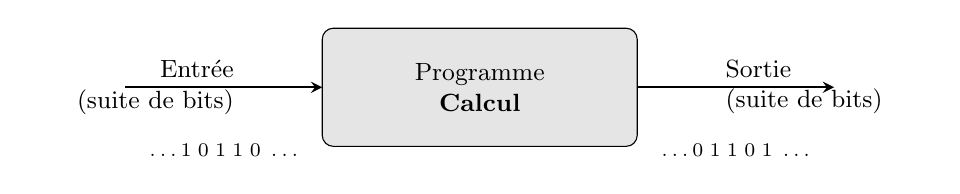
\begin{tikzpicture}[
    node distance=3cm, 
    every node/.style={font=\small},
    arrow/.style={->, thick, >=stealth}
]
    % Input label
    \node[anchor=east, align=right, text width=2.5cm] (input_label) at (-3,0) {
        Entrée \\ (suite de bits)
    };
    
    % Input arrow
    \draw[arrow] (-4.5,0) -- (-2,0);
    
    % Black box
    \node[
        draw,
        rectangle,
        rounded corners=4pt,
        minimum width=4cm,
        minimum height=1.5cm,
        align=center,
        fill=black!10
    ] (box) at (0,0) {
        Programme \\ \textbf{Calcul}
    };
    
    % Output arrow
    \draw[arrow] (2,0) -- (4.5,0);
    
    % Output label
    \node[anchor=west, align=left, text width=2.5cm] (output_label) at (3,0) {
        Sortie \\ (suite de bits)
    };
    
    % Example bit sequences (positioned below arrows)
    \node[font=\scriptsize] at (-3.25, -0.8) {
        $\ldots 1\;0\;1\;1\;0\;\ldots$
    };
    \node[font=\scriptsize] at (3.25, -0.8) {
        $\ldots 0\;1\;1\;0\;1\;\ldots$
    };
    
\end{tikzpicture}
\vspace{1em}

Nos entrées et sorties correspondent à des suites de bits,
on est dans le cadre discret.

On utilisera les symboles suivants:
\begin{itemize}
    \item L'alphabet: \(\Sigma = \left\{0,1\right\}\),
    \item L'ensemble des mots: \(\Sigma^*\),
\end{itemize}

On utilisera notamment les entiers à la place des mots. 
Pour ce faire, on veut une bijection entre \(\Sigma^*\) et \(\bb N\).
Problème? La fonction classique
\begin{equation*}
    x_1x_2\ldots x_n \mapsto \sum_{i=1}^n x_i 2^{i-1}
\end{equation*}
n'est pas une bijection car le mot \(00101\) et le mot \(101\) donnent le même entier.

On utilisera donc la méthode suivante:

Soit \(x_1,\ldots,x_n\) notre suite de bits. Pour la convertir en entier,
on commence par ajouter un 1 au début.
Donc la chaîne de bits \(x_1\ldots x_n\) devient
\(1x_1\ldots x_n\) mais problème, on ne peut pas coder le mot vide.
Pour régler ce problème, on fait moins 1.
Donc la chaîne de bits \(x_1\ldots x_n\) devient
\(1x_1\ldots x_n\) et on fait moins 1, et voilà
on a une bijection entre \(\Sigma^*\) et \(\bb N\).

Elle ressemble à ceci:
\begin{equation*}
    x_1x_2\ldots x_n \in \Sigma^* \mapsto \sum_{i=1}^n x_i 2^i - 1 \in \N
\end{equation*}


Pour appliquer un programme à une entrée 
on utilisera la notation non conventionnelle suivante:
\begin{equation*}
    \left[a\ \mid\ x\right]
\end{equation*}
qui représente l'exécution du programme \(a\) sur l'entrée \(x\).

On a alors deux possibilités:
\begin{itemize}
    \item Soit le programme s'arrête, et on note alors
        \(\left[a\mid x\right]\downarrow\) si le programme \(a\) sur l'entrée \(x\)
        s'arrête. On dit que ça converge.
    \item Soit le programme ne s'arrête pas, et on note alors
        \(\left[a\mid x\right]\uparrow\) si le programme \(a\) sur l'entrée \(x\)
        ne s'arrête pas. On dit que ça diverge.
    \item On note alors
        \(\left[a\mid x\right] = y\) si le programme \(a\) sur l'entrée \(x\)
        s'arrête et donne la sortie \(y\).
\end{itemize}

Il existe deux autres notations conventionnelles:
\begin{itemize}
    \item \(\varphi_a(x) = y\) si \(\left[a\mid x\right] = y\) (standard historique américain),

    \item \(U(a,x) = y\) si \(\left[a\mid x\right] = y\) (standard historique russe).
\end{itemize}

On pourra aussi utiliser \(\left[a\mid \cdot\right]\) pour désigner la fonction \defemph{partielle} suivante:
\begin{equation*}
    \begin{aligned}
        \left[a\mid \cdot\right]: \bb N &\to \bb N \\
        x &\mapsto \begin{cases}
            \left[a\mid x\right] & \text{si } \left[a\mid x\right]\downarrow, \\
            \text{non défini} & \text{si } \left[a\mid x\right]\uparrow.
        \end{cases}
    \end{aligned}
\end{equation*}

\begin{definition}
    Une fonction est \defemph{calculable} (ou récursive) si il existe un programme qui la calcule.
\end{definition}

On travaillera dans l'intégralité de ce cours (ou du moins ce chapitre) sur les entiers. 
On pourra donc dire \(\exists a\) sans préciser que \(a\) est un entier.


\begin{definition}
    La \defemph{fonction caractéristique} d'un ensemble \(A\subseteq \bb N\) est la fonction
    \begin{equation*}
        \chi_A: \bb N \to \left\{0,1\right\}, \quad x \mapsto \begin{cases}
            1 & \text{si } x\in A, \\
            0 & \text{sinon}.
        \end{cases}
    \end{equation*}
\end{definition}

\begin{definition}
    Un ensemble \(A\subseteq \bb N\) est \defemph{décidable} (ou \defemph{récursif}) si sa fonction caractéristique \(\chi_A\) est calculable.
\end{definition}

\begin{definition}
    Un ensemble \(A\subseteq \bb N\) est \defemph{énumérable} (ou \defemph{récursivement énumérable}) si il est le domaine d'une fonction calculable.

    D'autres mots pour dire la même chose:
    \begin{itemize}
        \item récursivement énumérable,
        \item calculatoirement énumérable,
        \item semi-décidable (à ne pas utiliser).
    \end{itemize}
\end{definition}

\begin{definition}
    Le \defemph{domaine} d'une fonction \(a\) est l'ensemble
    \begin{equation*}
        \text{dom}(a) = \left\{x\in \bb N \mid [a\mid x] \downarrow \right\}
    \end{equation*}
\end{definition}

\begin{theorem}[de Post]
    Soit \(E\subseteq \bb N\). Si \(E\) et \(\ol{E}\) sont énumérables, alors \(E\) est décidable 
    (où \(\ol{E} = \bb N \setminus E\) est le complémentaire de \(E\) dans \(\bb N\))
\end{theorem}

\begin{proof}
    Soit \(E\subseteq \bb N\) tel que \(E\) et \(\ol{E}\) sont énumérables.
    Donc il existe des programmes \(a\) et \(b\) tels que
    \(\text{dom} [a \mid \cdot] = E\) et \(\text{dom} [b \mid \cdot] = \ol{E}\).
    On veut construire un programme \(c\) qui décide \(E\).
    On utilise la fonction \(\text{Step}\) de la manière suivante:
    \begin{align*}
        \text{Step}\langle a,x,t \rangle &= \begin{cases}
            0 & \text{si } a \text{ n'a pas terminé après } t \text{ étapes sur l'entrée } x, \\
            1 + [a \mid x] & \text{sinon}.
        \end{cases} \\
    \end{align*}

    Ensuite, on utilise la fonction \(\text{Step}\) pour construire le programme \(c\) qui décide \(E\):
    \begin{align*}
        c: x \mapsto\ & t \leftarrow 0 \\
        & \text{tant que } \text{Step}\langle a,x,t \rangle = 0 \text{ et } \text{Step}\langle b,x,t \rangle = 0 \\
        & \quad t \leftarrow t + 1 \\
        & \text{si } \text{Step}\langle a,x,t \rangle \neq 0 \text{ alors return } 1 \\
        & \text{sinon return } 0
    \end{align*}
    Donc \(E\) est décidable.
\end{proof}
